\section{POSIX Overheads}
\label{sec:posix-overheads}

\begin{figure}[tb]
\centering
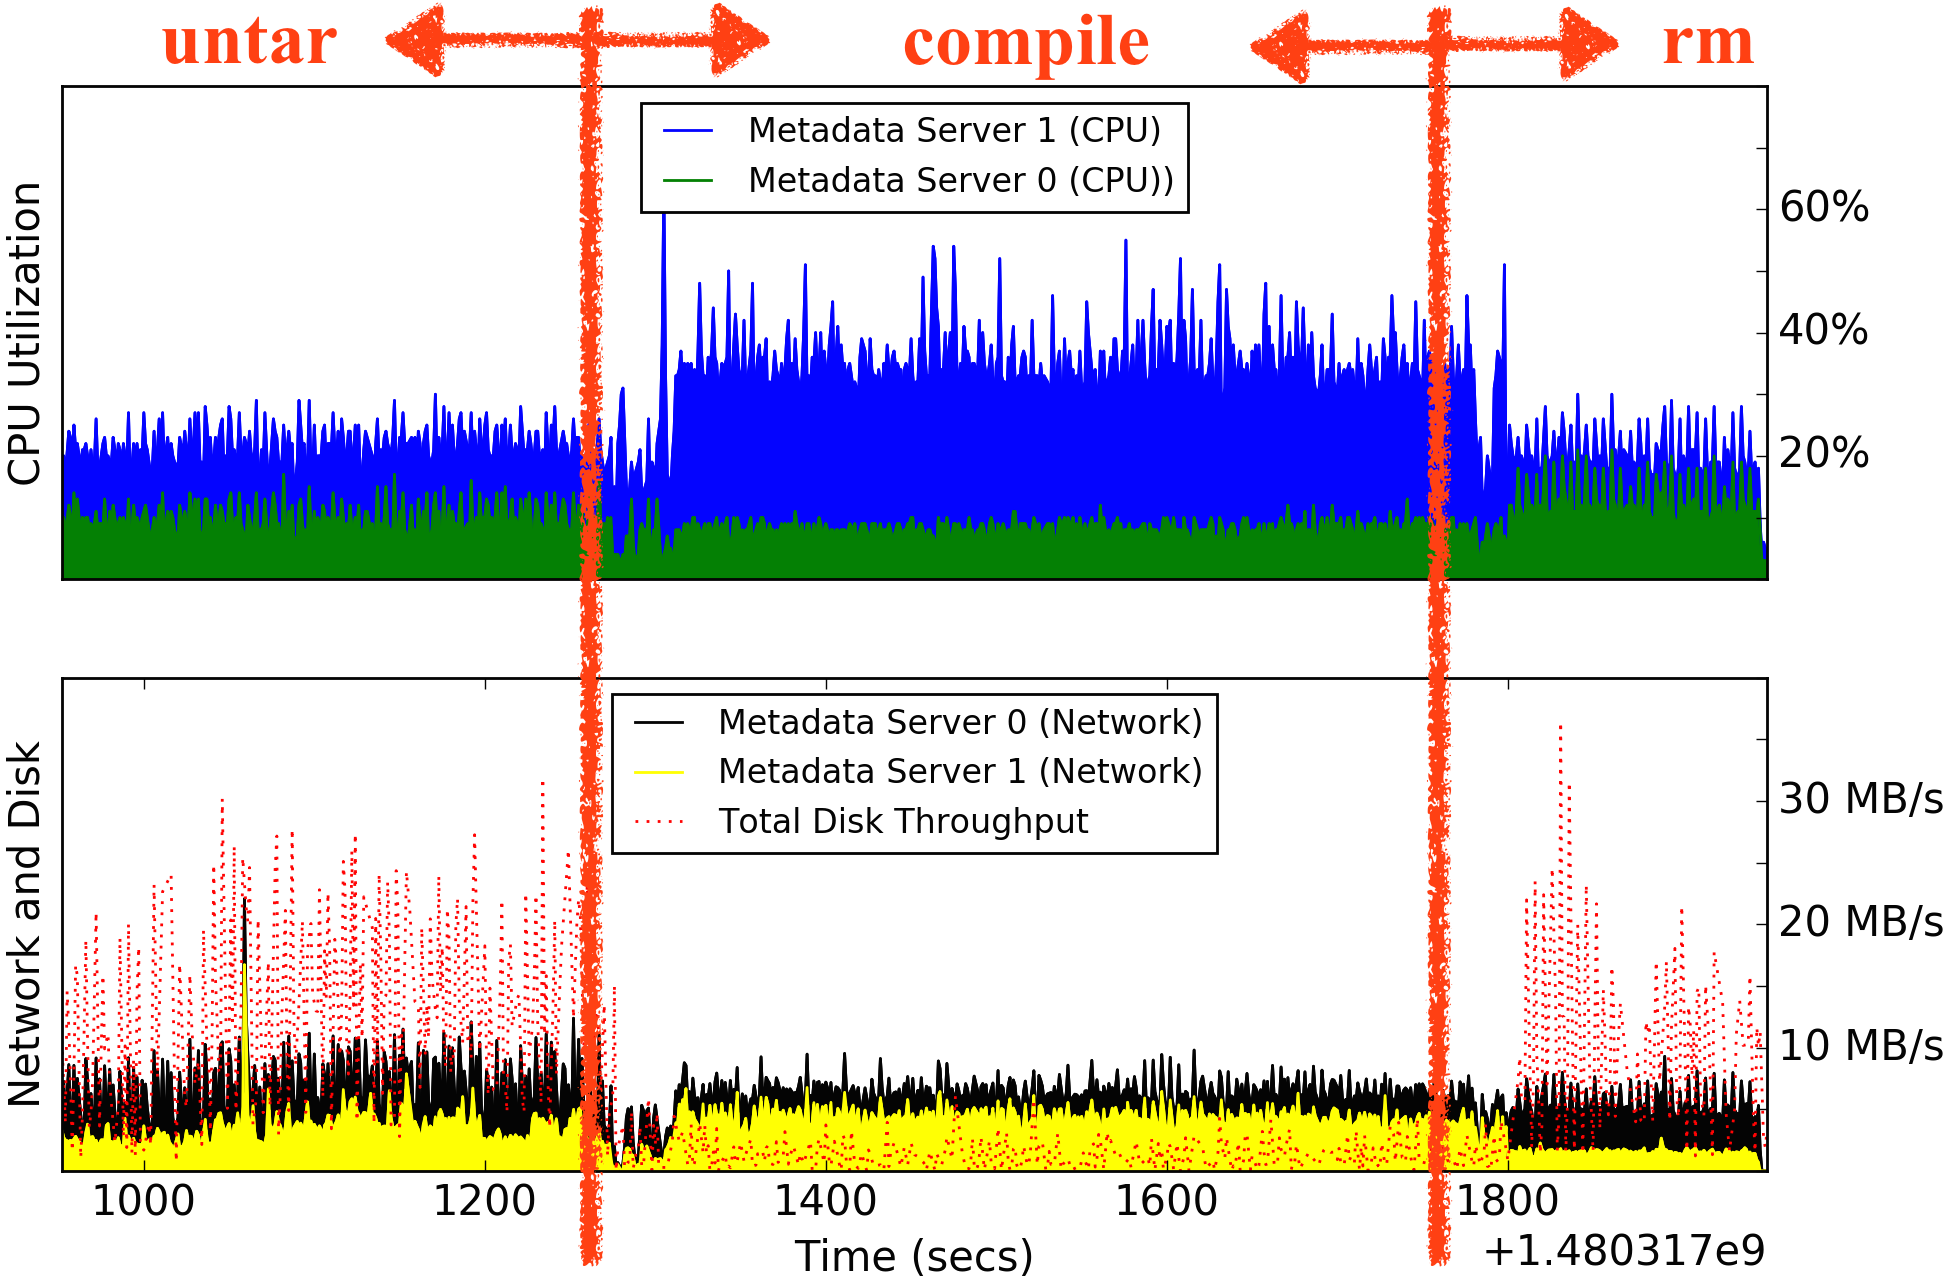
\includegraphics[width=1\linewidth]{./graphs/overhead-creates.png}
\caption{Create-heavy workloads (such as \texttt{untar}) incur the highest disk, network, and
CPU utilization because of the consistency and durability demands of
CephFS.}\label{fig:overhead-creates}
\end{figure}

In our examination of the overheads of POSIX we benchmark and analyze CephFS,
the file system that uses the Ceph's object store ({\it i.e.} RADOS) to store
its data and metadata. We choose CephFS because it is an open-source production
quality system. This file system is an implementation of one set of design
decisions and our goal is to highlight the effect that those decisions have on
performance.

To show how the file system behaves under high metadata load we use a
create-heavy workload. Create-heavy workloads are studied the most in HPC
research because of the checkpoint/restart use case but they also happen to
stress the underlying storage system the most.
Figure~\ref{fig:overhead-creates} shows the resource utilization of compiling
the Linux kernel.  The \texttt{untar} phase, which is characterized by many creates, has
the highest resource usage which suggests that it is stressing the consistency
and journaling subsystems of the metadata server the most. Traditional file
system techniques for improving performance, such as caching inodes, do not
help for create-heavy workloads.

\begin{figure}[tb]
\centering
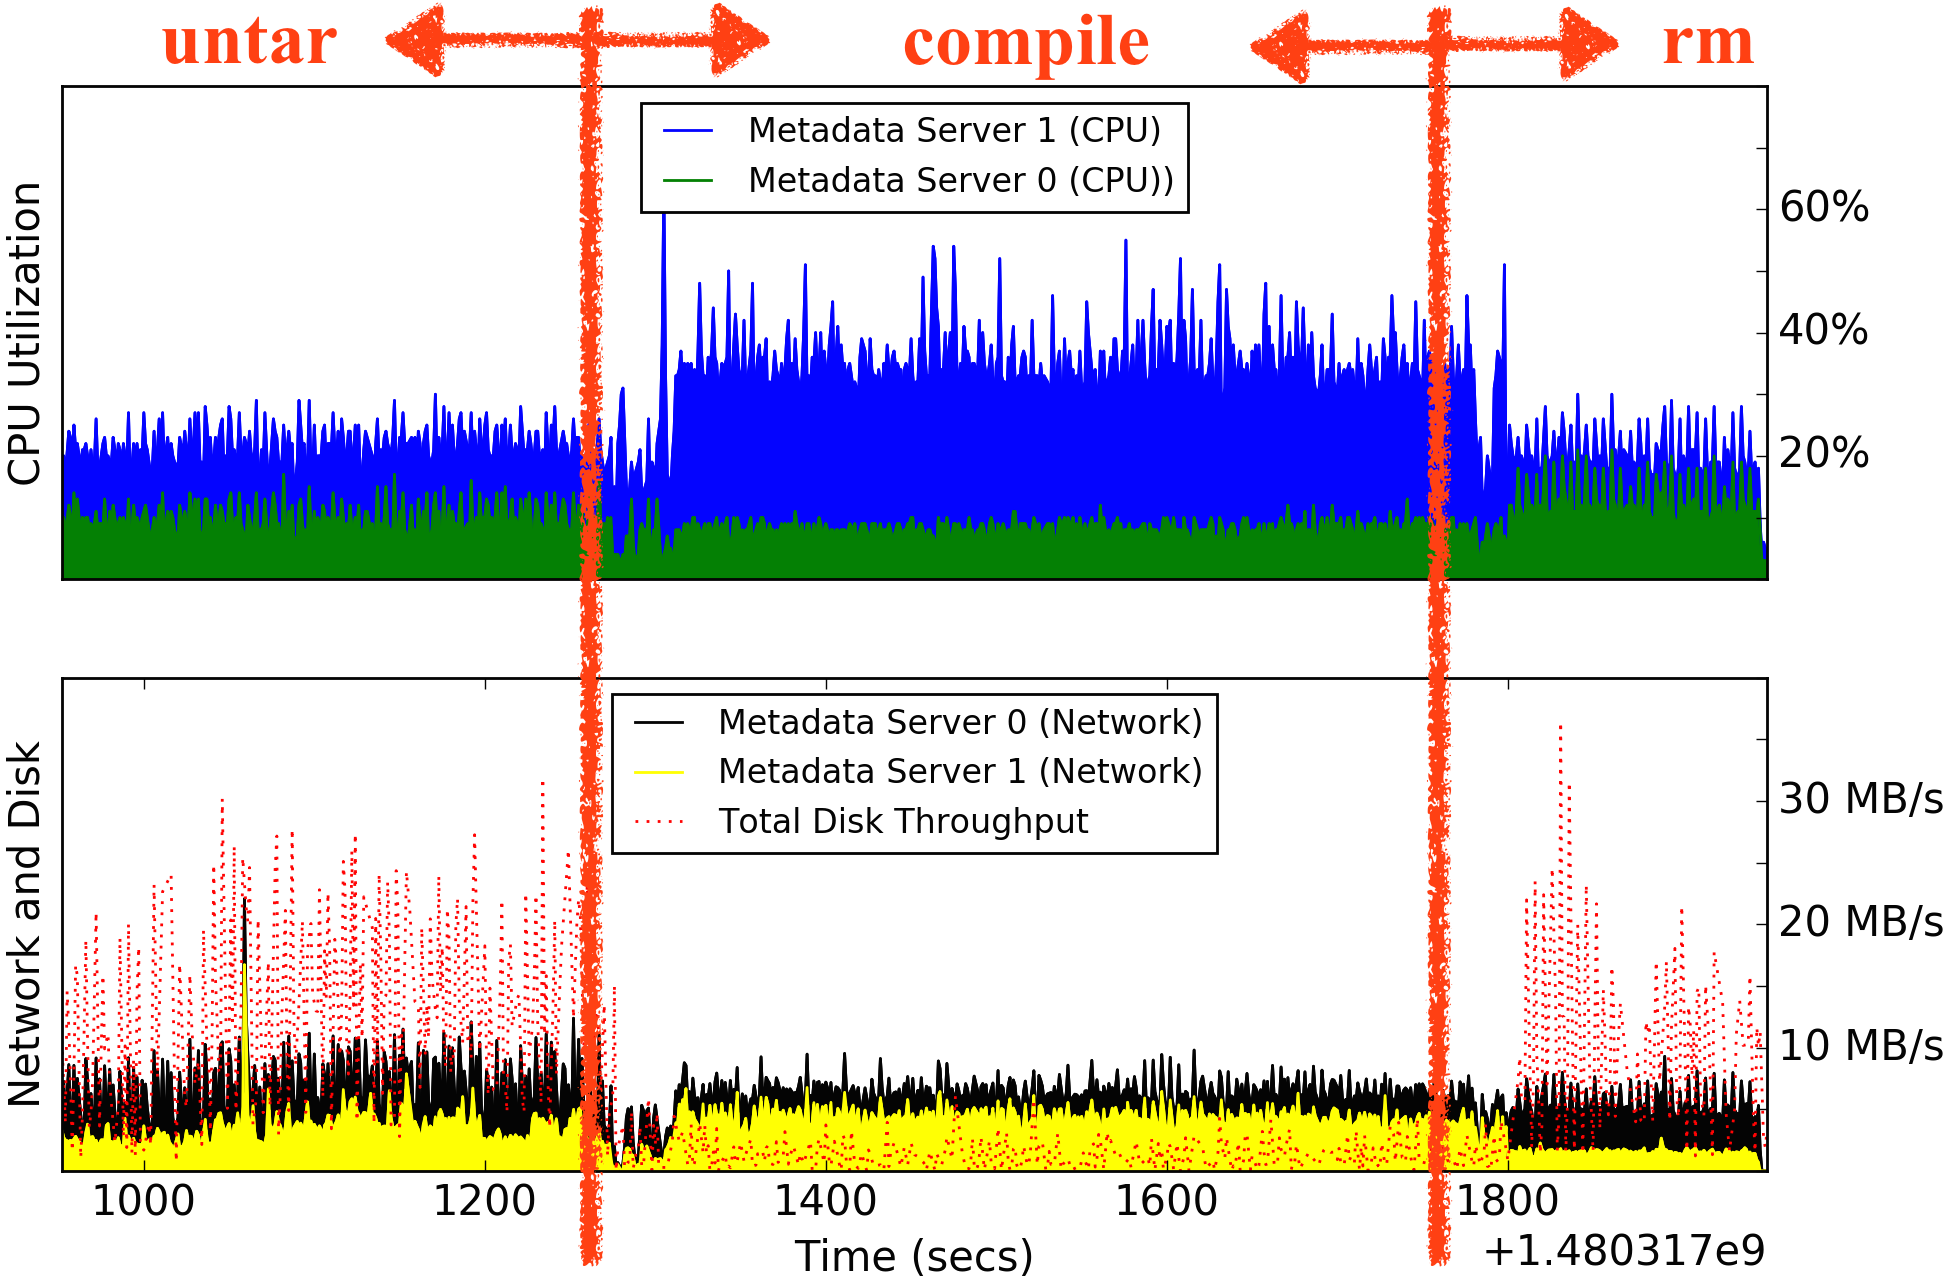
\includegraphics[width=1\linewidth]{./graphs/overhead-creates.png}
\caption{Create-heavy workloads (untar) incurr the highest disk, network, and
CPU utilization because of the consistency and durability demands of
CephFS.}\label{fig:overhead-creates}
\end{figure}

In this section, we quantify the costs of strong consistency and global
durability in CephFS. At the end of each subsection we compare the approach to
``decoupled namespaces", the technique in related work that detaches subtrees
from the global namespace to relax consistency/durability guarantees.  We use
the kernel client so that we can find the true create speed of the server; our
experiments show a low CPU utilization for the clients which indicates that we
are stressing the servers more.

\subsection{Durability}
\label{sec:durability}

% what is durability
While durability is not specified by POSIX, users expect that files they create
or modify survive failures.  We define three types of durability: global,
local, and none.  Global
durability means that the client or server can fail at any time and metadata
will not be lost. Local durability means that metadata can be lost if the
client or server stays down after a failure. None means that metadata is volatile
and that the system provides no guarantees when clients or servers fail. 
None is different than local durability because regardless of the type failure,
metadata will be lost when components die in a None configuration.\\

% - sequential IO, trim redundant operations
\noindent\textbf{CephFS Design}: a journal of metadata updates that streams into
the resilient object store. Similar to LFS~\cite{rosenblum:acm1992-LFS} and
WAFL~\cite{hitz:wtec1994-WAFL} the metadata journal is designed to grow to large which
ensures (1) sequential writes into the object store and (2) the ability for daemons to
trim redundant or irrelevent journal entries.  The journal is striped over
objects where multiple journal updates can reside on the same object. There are
two tunables for controlling the journal: the segment size and the number of
parallel segments that can be written in parallel. Unless the journal saturates 
memory or CPU resources, larger values for these tunables results in better
performance.

% purpose of the journal
As shown in Figure~\ref{fig:journal}, in addition to the metadata journal,
CephFS also represents metadata in RADOS as a metadata store, where directories
and their file inodes are stored as objects.  The metadata server applies the
updates in the journal to the metadata store when the journal reaches a certain
size. The metadata store is optimized for recovery ({\it i.e.} reading) while
the metadata journal is write-optimized.

\begin{figure}[tb] \centering
\includegraphics[width=1\linewidth]{./figures/journal.png} 
\caption{CephFS uses a journal to stage updates and tracks dirty metadata in
the collective memory of the metadata servers. Each metadata server maintains its own journal, which is
broken up into 4MB segments. These segments are pushed into RADOS and deleted
when that particular segment is trimmed from the end of the log. In addition to
journal segments, RADOS also stores per-directory objects. \label{fig:journal}}
\end{figure}
\begin{figure*}[t]
  \centering
  \begin{subfigure}[b]{.3\linewidth}
      \centering
      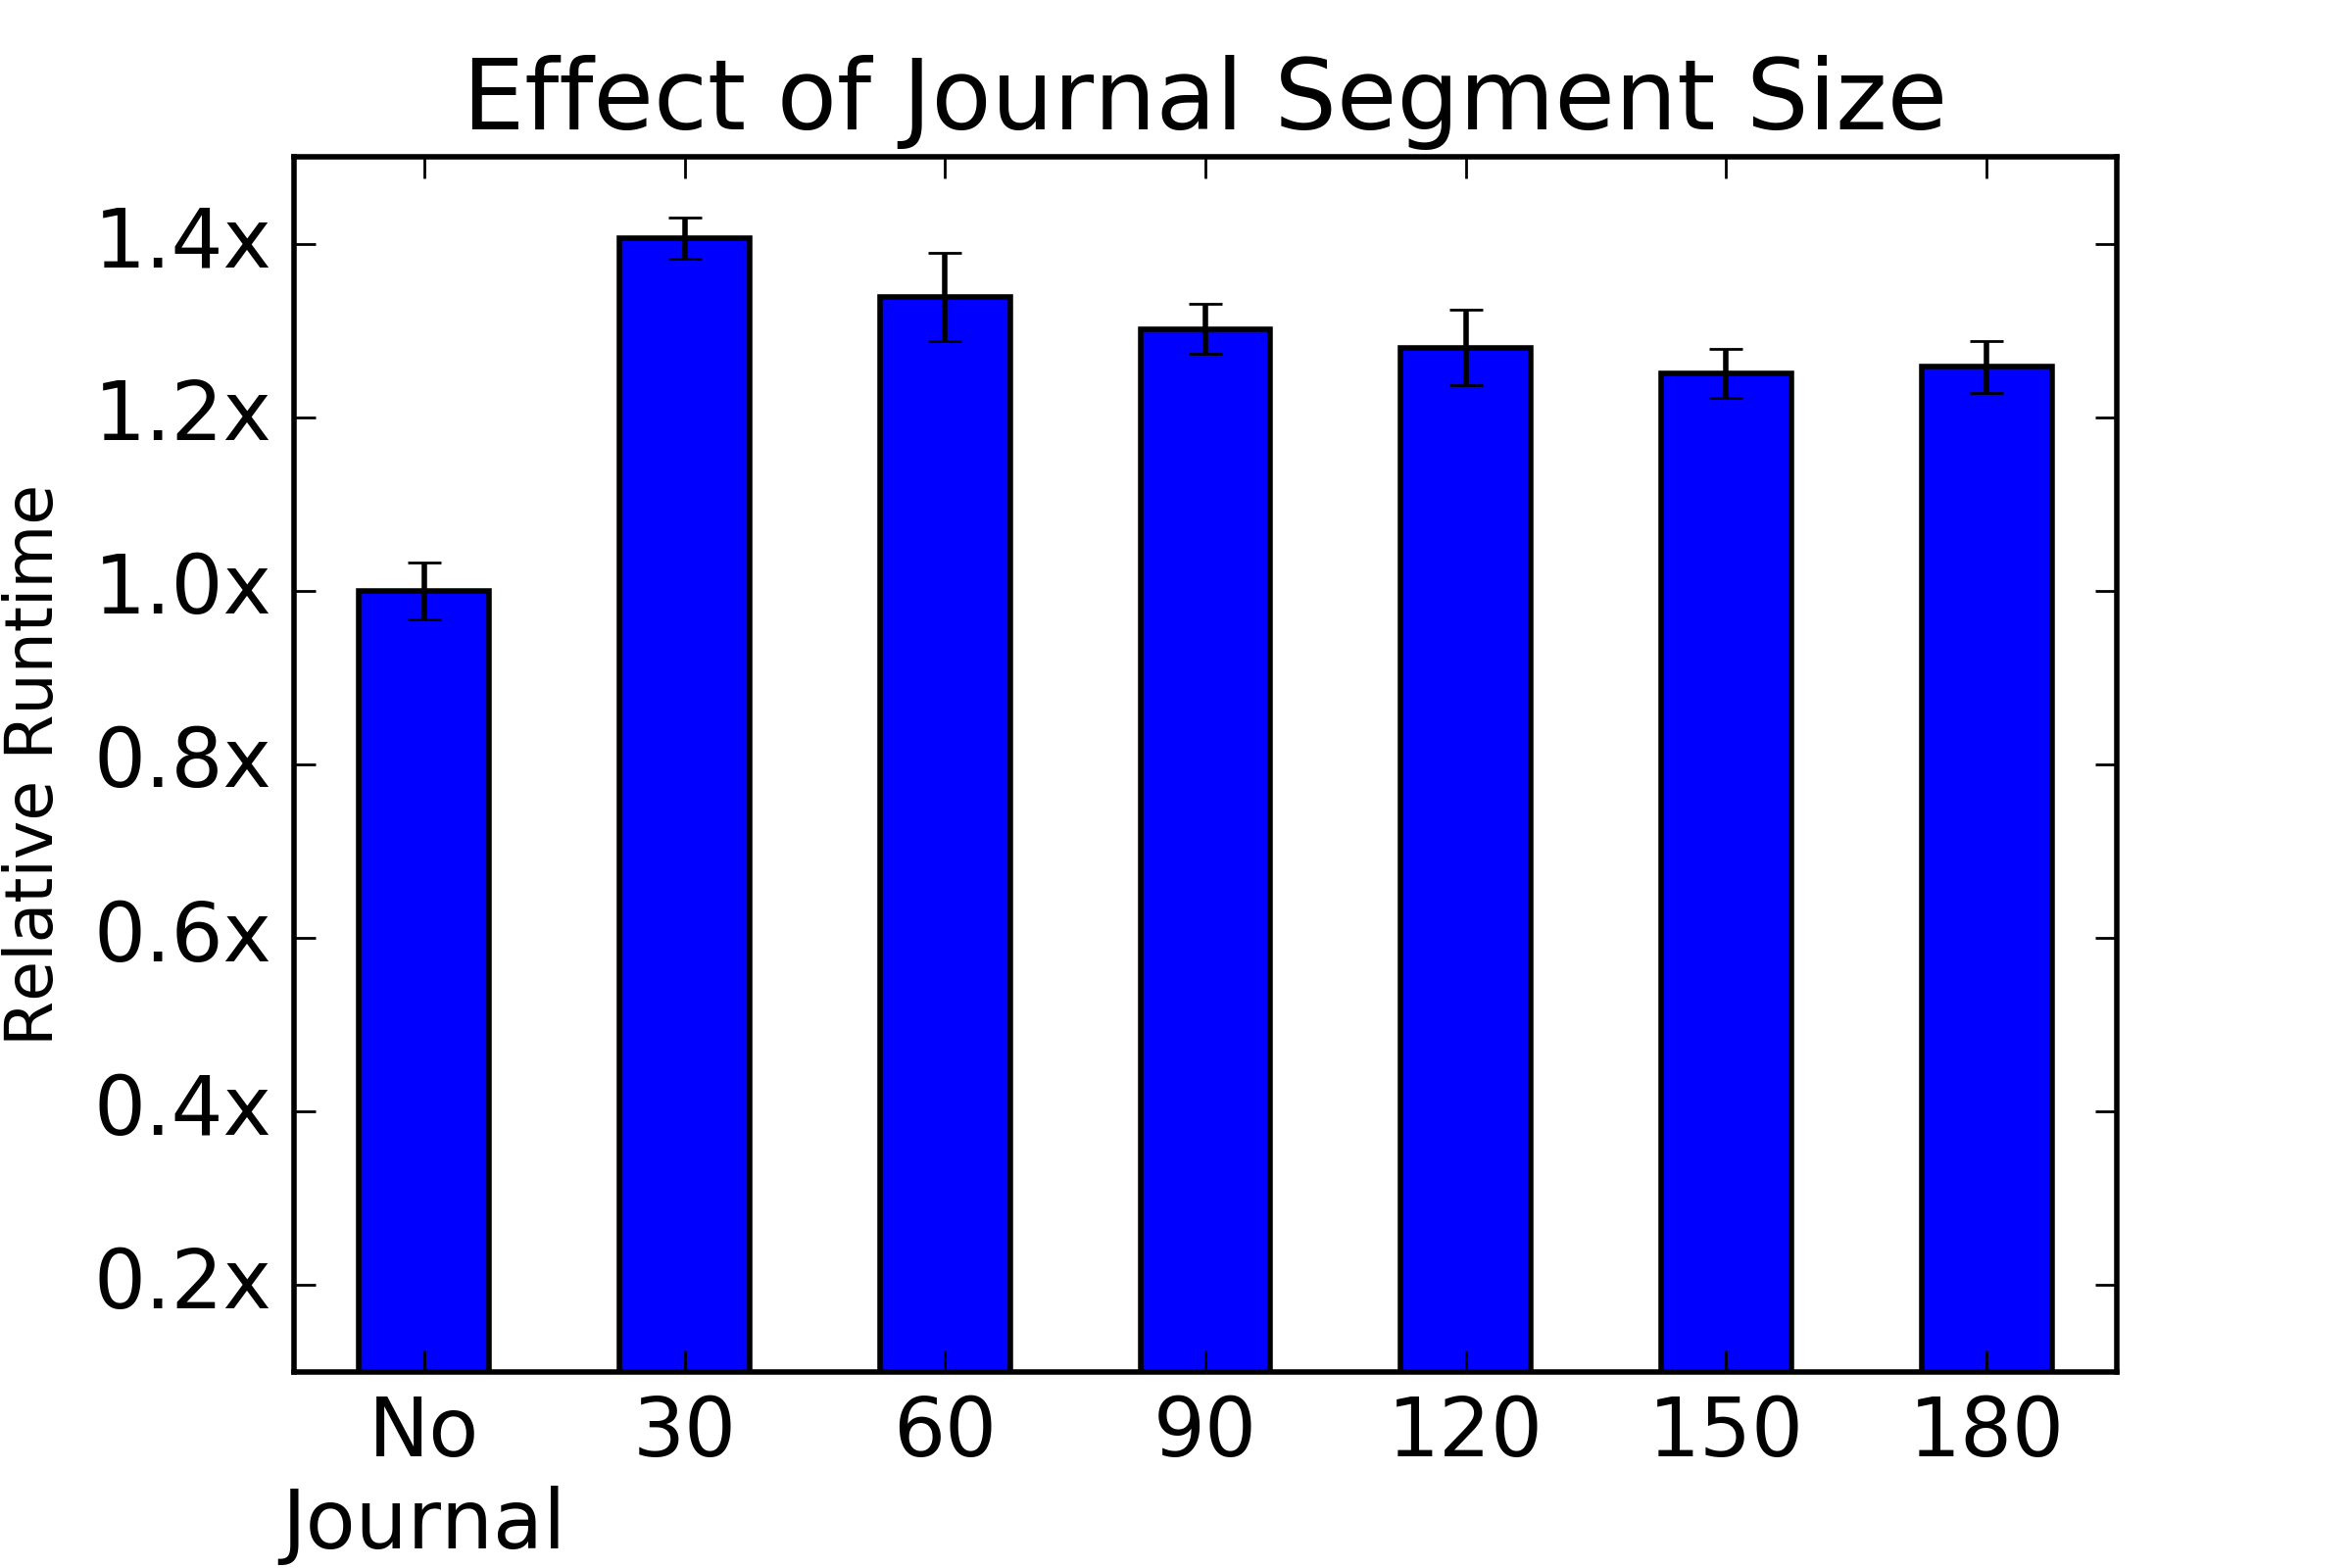
\includegraphics[width=1.0\linewidth]{graphs/slowdown-journal.png}
      \caption{Journal Segment Size} \label{fig:slowdown-journal-a}
  \end{subfigure}
  \begin{subfigure}[b]{.3\linewidth}
      \centering
      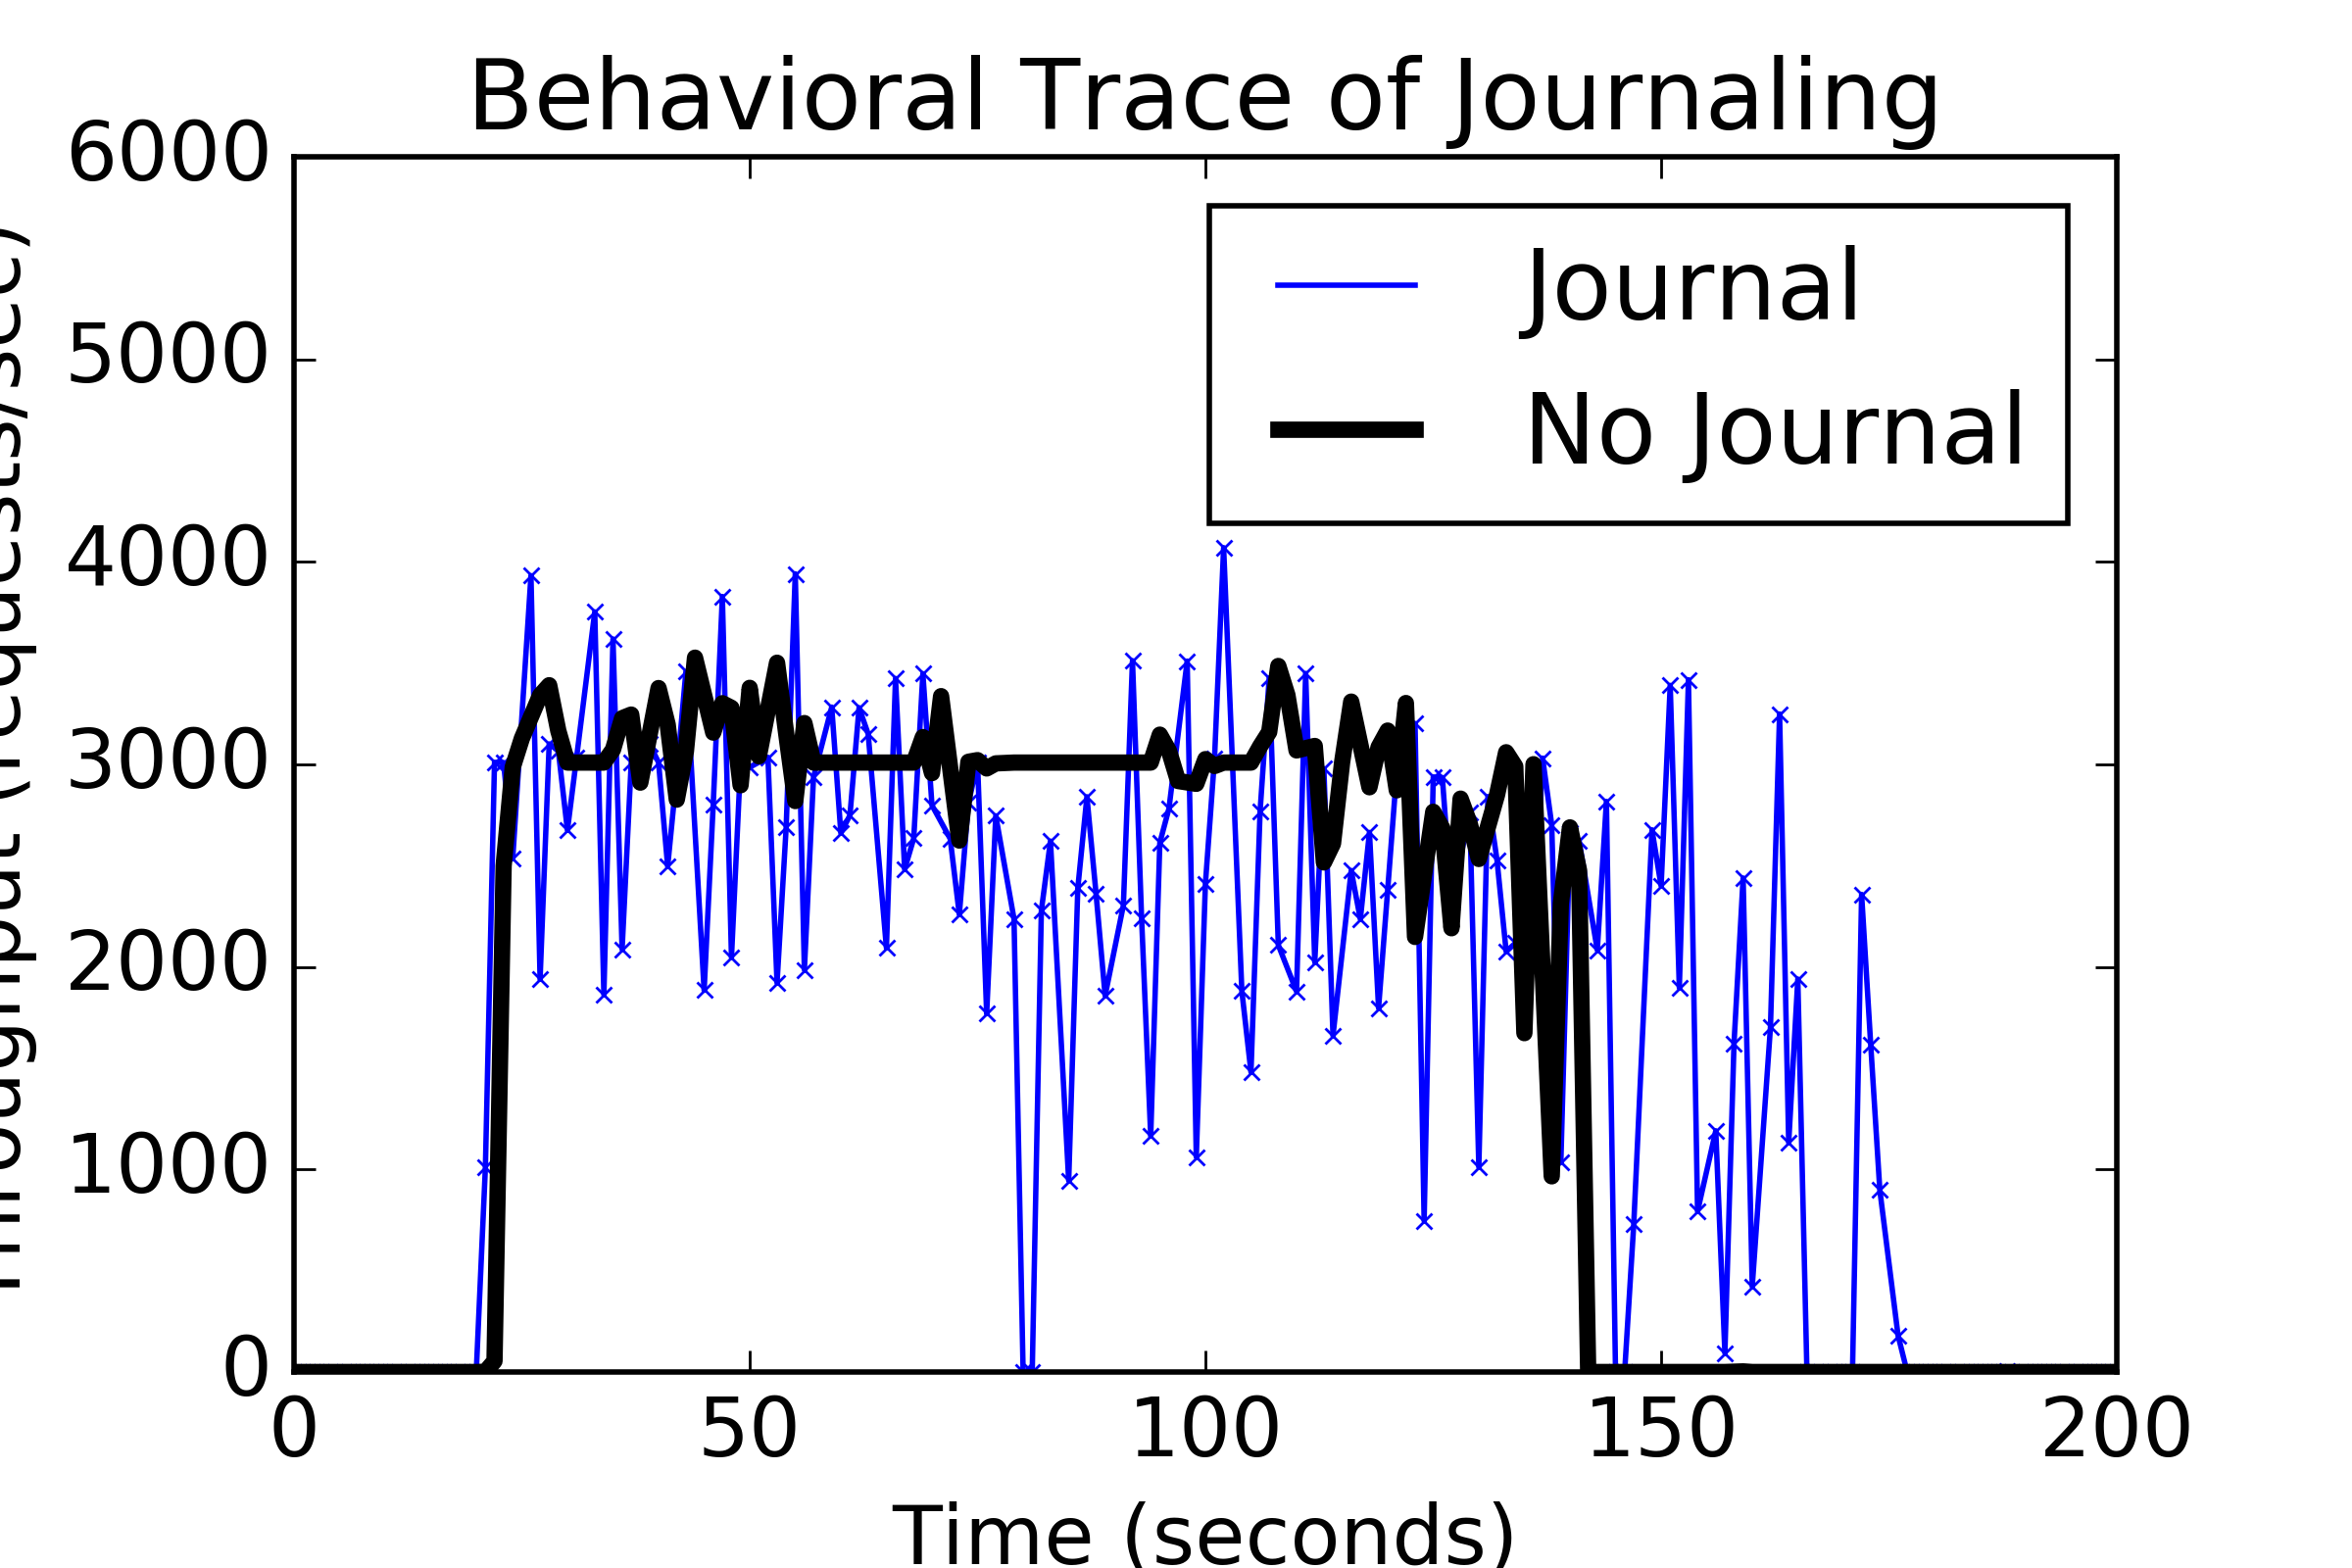
\includegraphics[width=1.0\linewidth]{graphs/behavior-journal.png}
      \caption{180MB Segment vs. No Journal}
      \label{fig:slowdown-journal-b}
  \end{subfigure}
  \begin{subfigure}[b]{.3\linewidth}
      \centering
      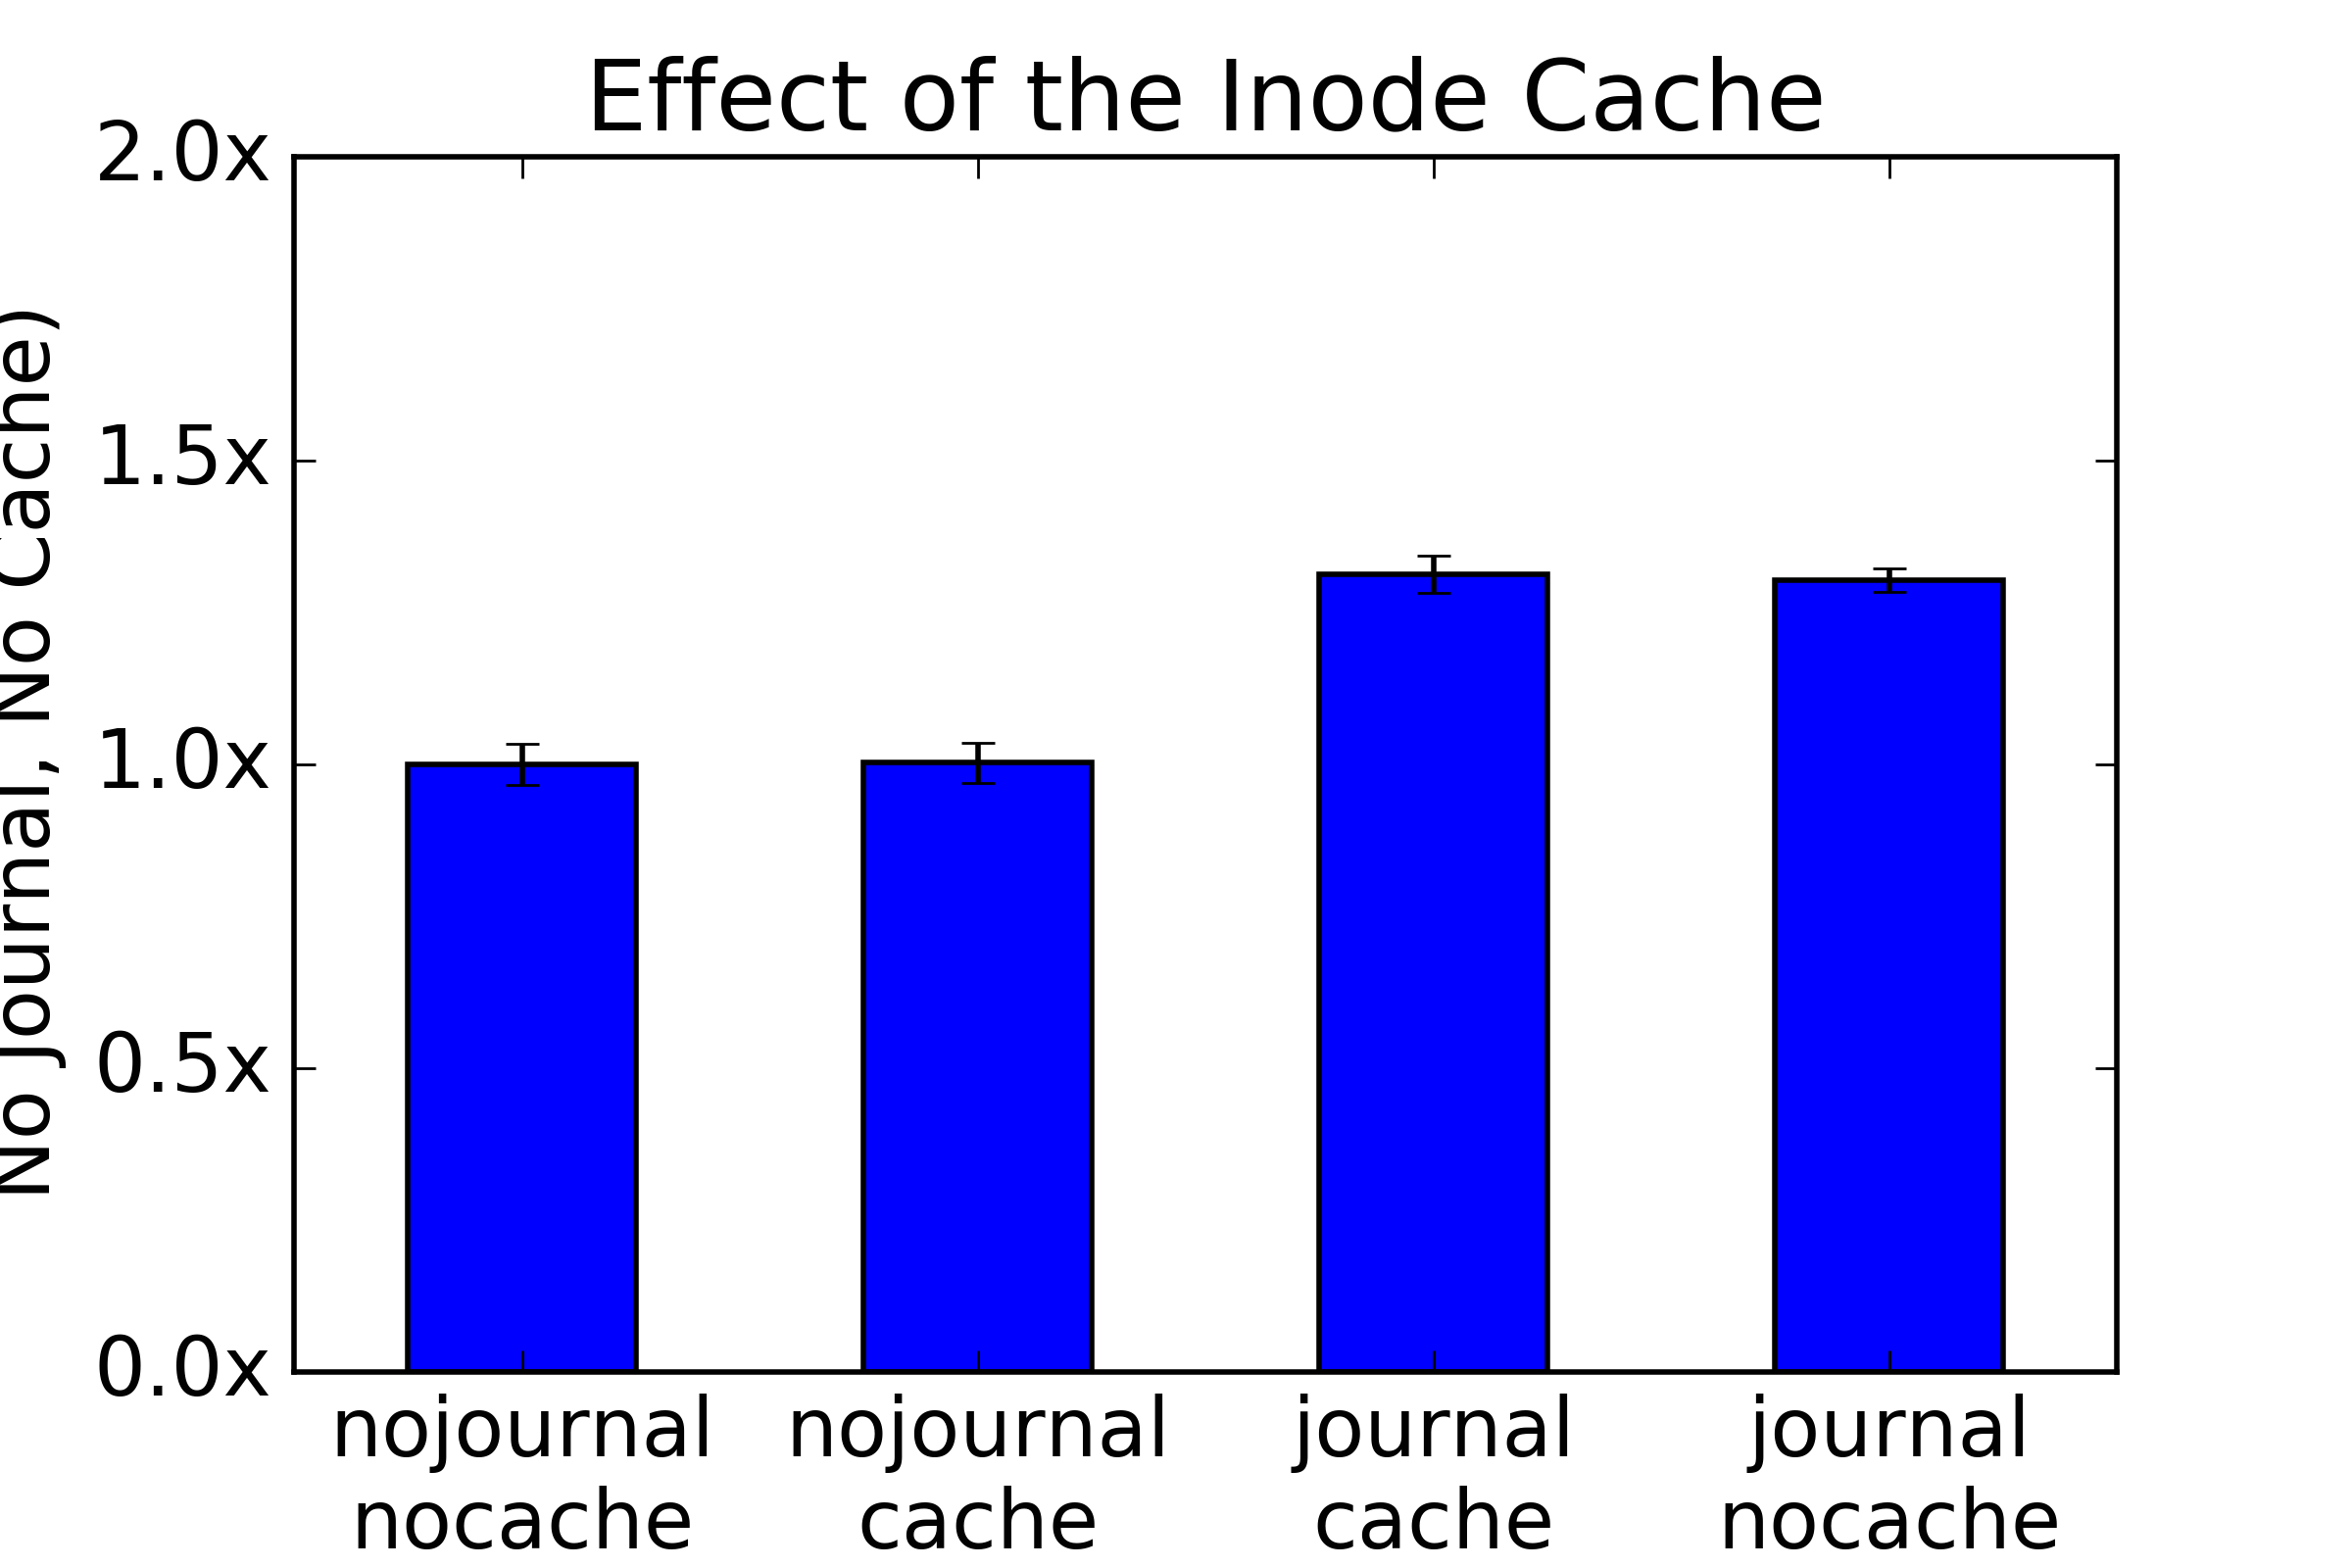
\includegraphics[width=1.0\linewidth]{graphs/slowdown-cache.png}
      \caption{Inode Cache}
      \label{fig:slowdown-journal-c}
  \end{subfigure}
  \caption{The overhead of the file system metadata journal. The segment size
  is the threshold that the metadata server starts
  trimming.\label{fig:slowdown-journal}}
\end{figure*}

% what is durability
While durability is not specified by POSIX, users expect that files they create
or modify survive failures.  We define three types of durability: global,
local, and none.  Global
durability means that the client or server can fail at any time and metadata
will not be lost. Local durability means that metadata can be lost if the
client or server stays down after a failure. None means that metadata is volatile
and that the system provides no guarantees when clients or servers fail. 
None is different than local durability because regardless of the type failure,
metadata will be lost when components die in a None configuration.\\

% - sequential IO, trim redundant operations
\noindent\textbf{CephFS Design}: a journal of metadata updates that streams into
the resilient object store, similar to LFS~\cite{rosenblum:acm1992-LFS} and
WAFL~\cite{hitz:wtec1994-WAFL}, grows to large extents which
allows to (1) sequentially write into the object store and (2) provide the ability for daemons to
trim redundant or irrelevant journal entries.  The journal is striped over
objects where multiple journal updates can reside on the same object. There are
two tunables for controlling the journal: the segment size and the number of
parallel segments that can be written in parallel. Unless the journal saturates 
memory or CPU resources, larger values for these tunables results in better
performance.

% purpose of the journal
As shown in Figure~\ref{fig:journal}, in addition to the metadata journal,
CephFS also stores metadata in RADOS, where directories
and their file inodes are stored as objects.  The metadata server applies the
updates in the journal to this metadata store when the journal reaches a certain
size. The metadata store is optimized for recovery ({\it i.e.} reading) while
the metadata journal is write-optimized.

% Effects on performance
Figure~\ref{fig:slowdown-journal} shows that journaling metadata updates into
the object store has an overhead. Figure~\ref{fig:slowdown-journal-a} shows the
effect of journaling of different journal segment sizes; the larger the segment
size the bigger that the writes into the object store are. The trade-off for
better performance is memory consumption because larger segments take up
more space for buffering. Figure~\ref{fig:slowdown-journal-b} shows how
the metadata server periodically stops serving requests to flush ({\it i.e.}
apply journal updates to) to the metadata store.  The journal overhead is
sufficient enough to slow down metadata throughput but not so much as to
overwhelm the bandwidth of the object store. We measured our peak bandwidth to
be 100MB/s, which is the speed of our network link.\\

\noindent\textbf{Comparison to decoupled namespaces}: In BatchFS and DeltaFS,
to the best of our knowledge, when a client or server fails there is no recovery
scheme. For BatchFS, if a client fails when it is writing to the local
log-structured merged tree (implemented as an SSTable) then those batched
metadata operations are lost. For DeltaFS, if the client fails then, on restart,
the computation does the work again -- since the snapshots of the namespace are
never globally consistent and there is no ground truth.  On the server side,
BatchFS and DeltaFS use IndexFS. IndexFS writes metadata to SSTables, which
initially reside in memory but are later flushed to the underlying
distributed file system.

\subsection{Strong Consistency}
\label{sec:strong-consistency}

Access to metadata in a POSIX-compliant file system is strongly consistent, so
reads and writes to the same inode or directory are globally ordered.  The
synchronization and serialization machinery needed to ensure that all clients
see the same state has high overhead.\\

\noindent\textbf{CephFS Design}: capabilities keep metadata strongly
consistent. To reduce the number of RPCs needed for consistency, clients can
obtain capabilities for reading, creating and updating inodes, as well as caching reads,
buffering writes, changing the file size, and performing lazy IO.

\begin{figure*}[t]
  \centering
  \begin{subfigure}[b]{.3\linewidth}
      \centering
      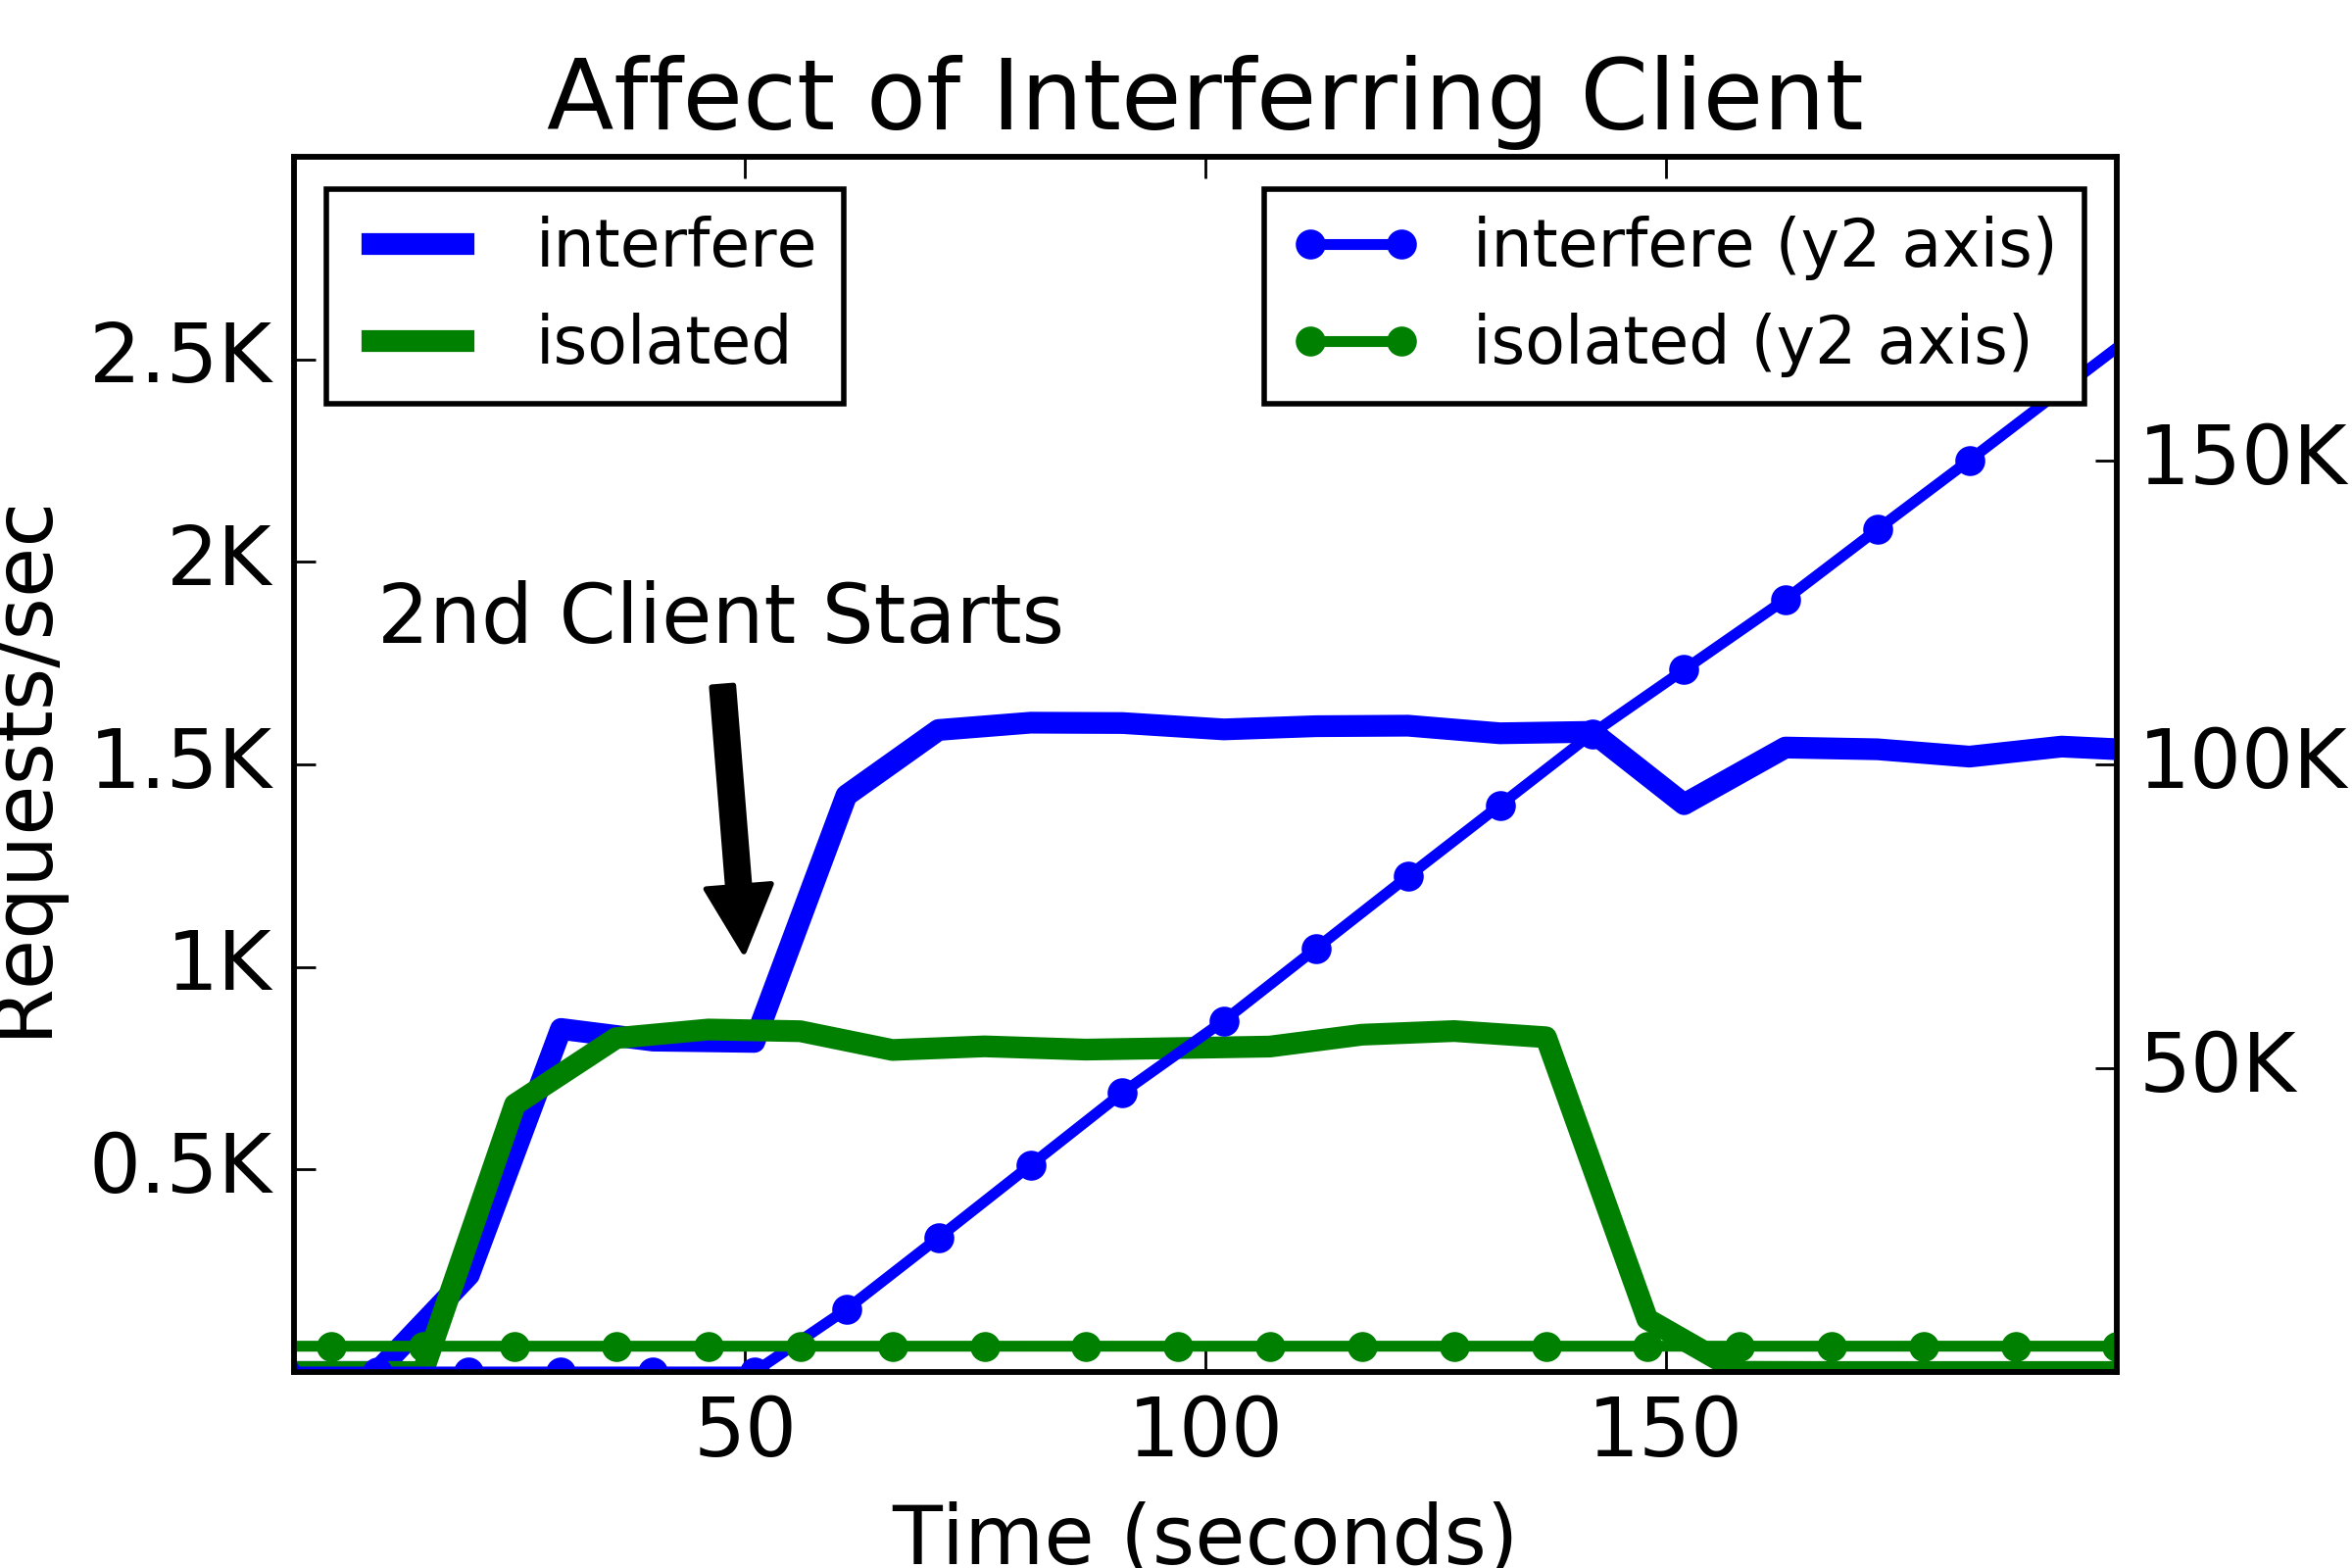
\includegraphics[width=1.0\linewidth]{graphs/behavior-interfere.png}
      \caption{Inteference forces \texttt{lookup()}s}
      \label{fig:interfere-a}
  \end{subfigure}
  \begin{subfigure}[b]{.3\linewidth}
      \centering
      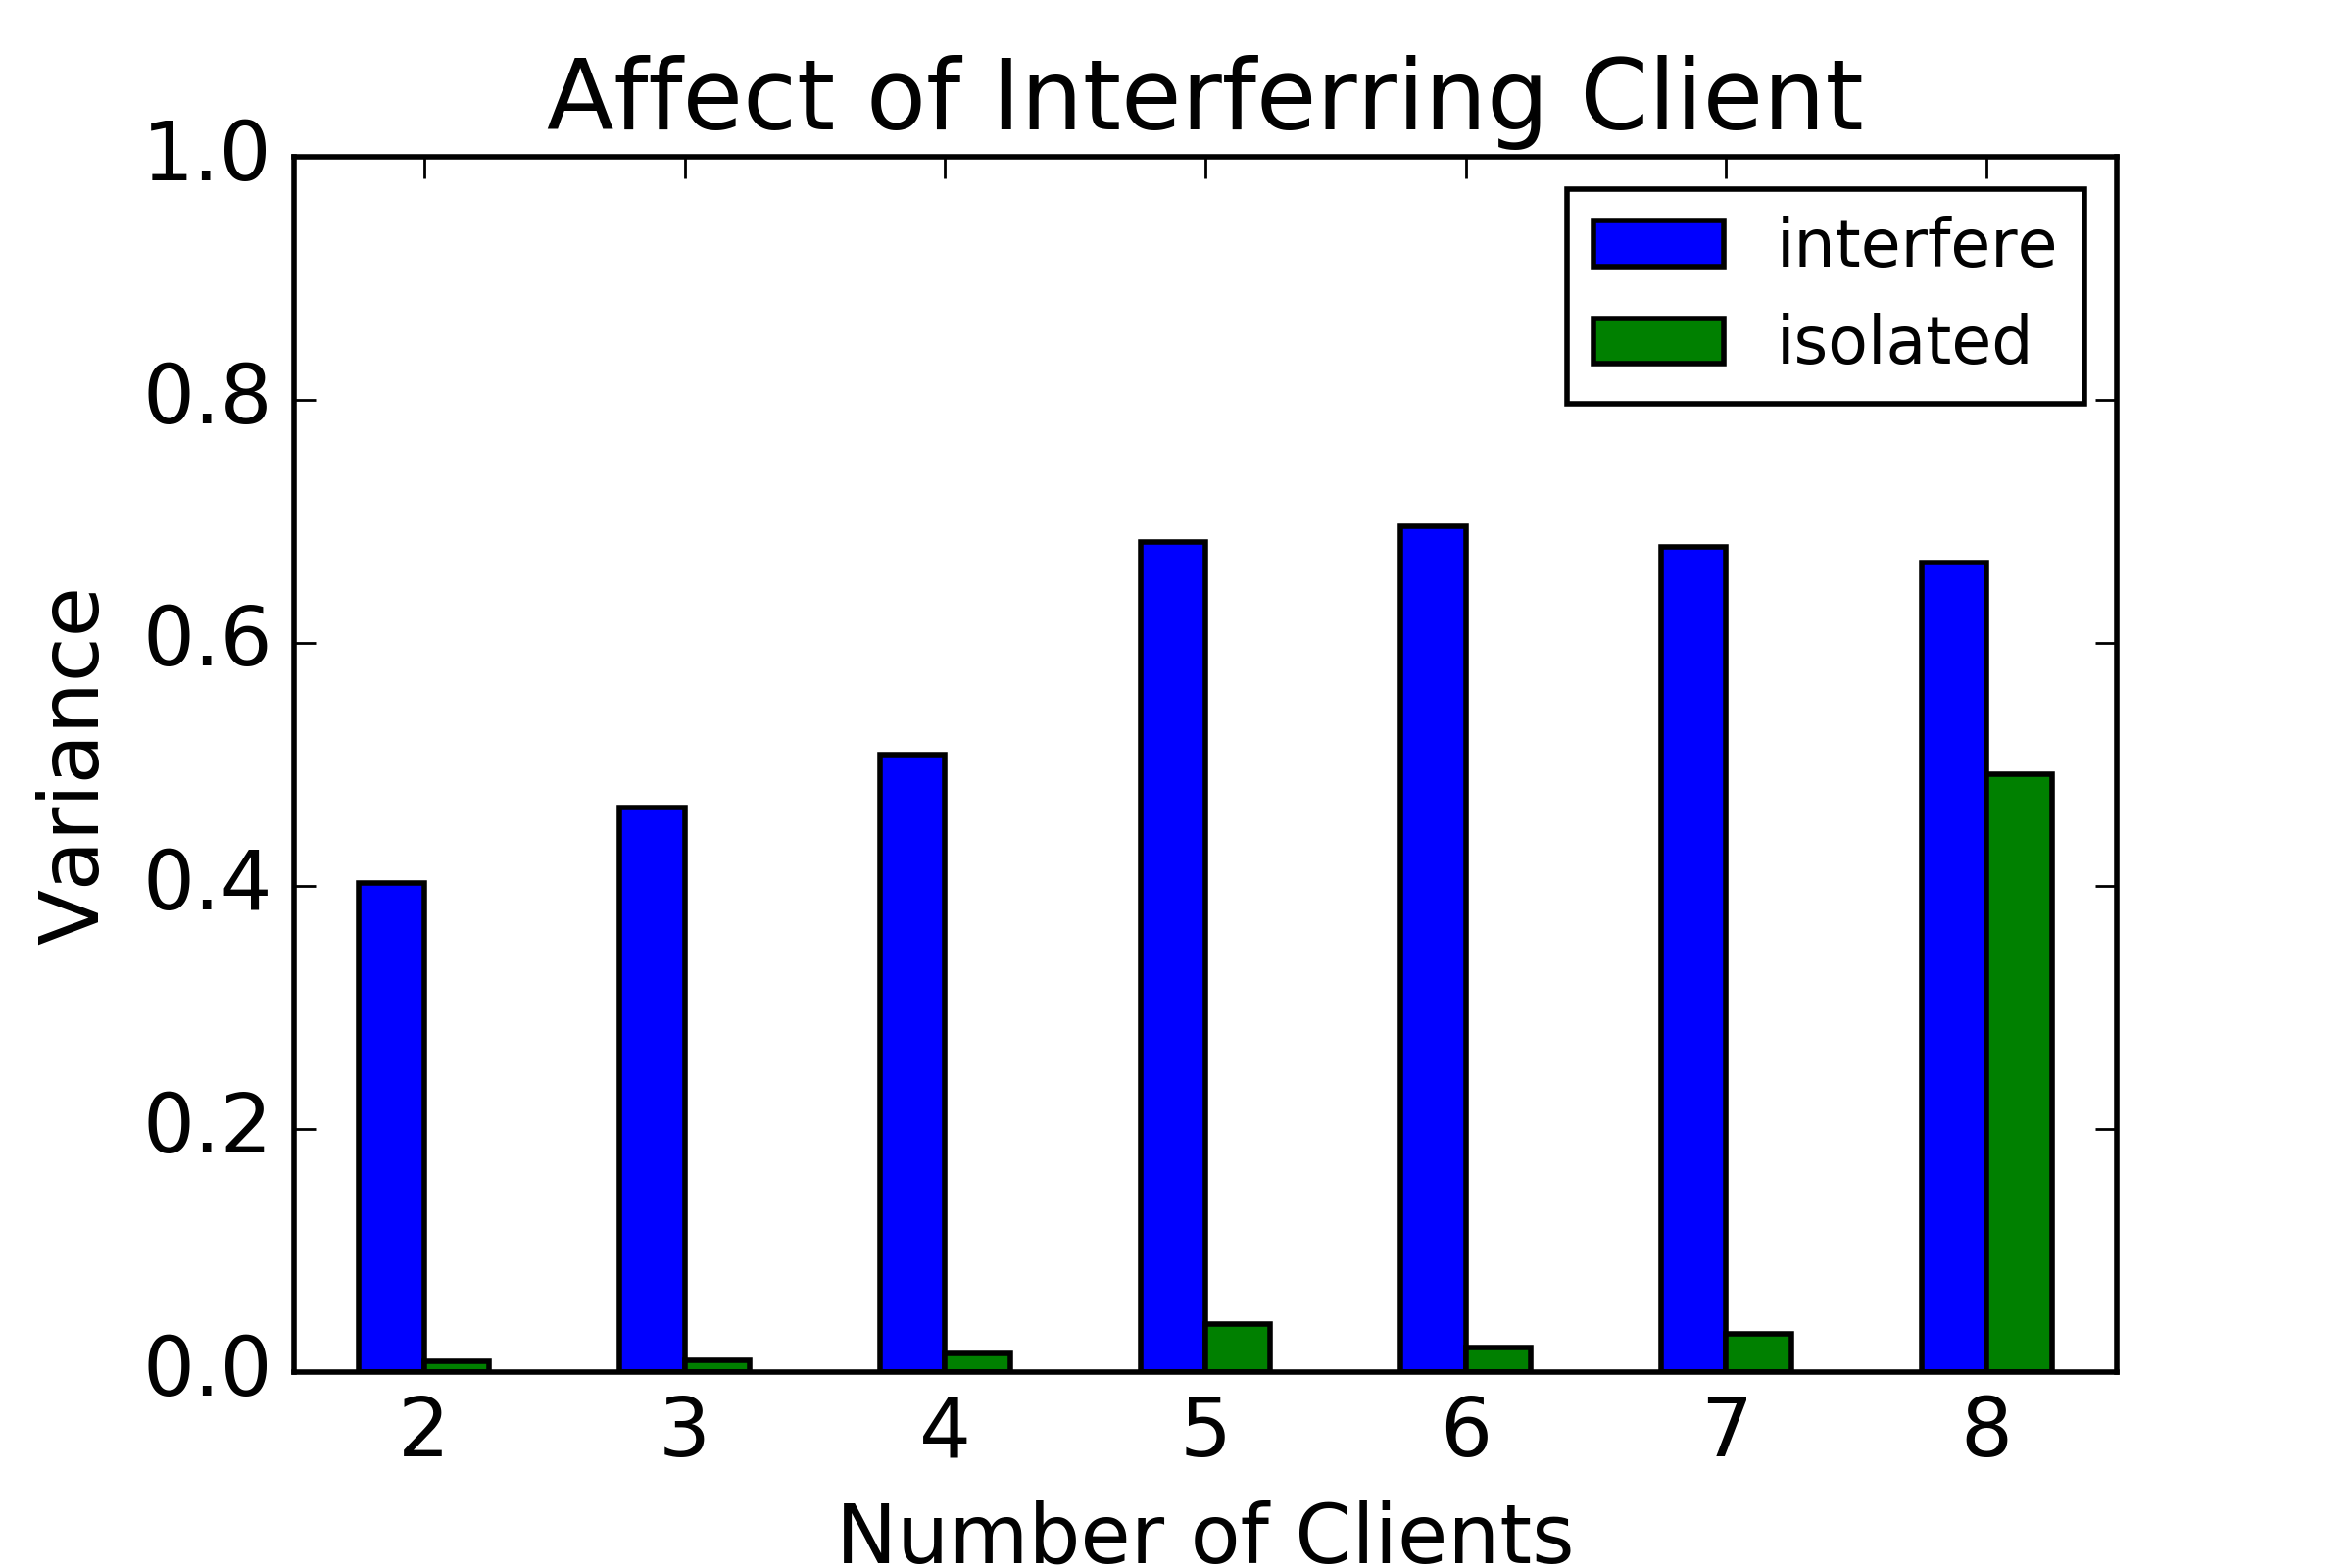
\includegraphics[width=1.0\linewidth]{graphs/slowdown-interfere.png}
      \caption{Interference hurts performance}
      \label{fig:interfere-b}
  \end{subfigure}
  \begin{subfigure}[b]{.3\linewidth}
      \centering
      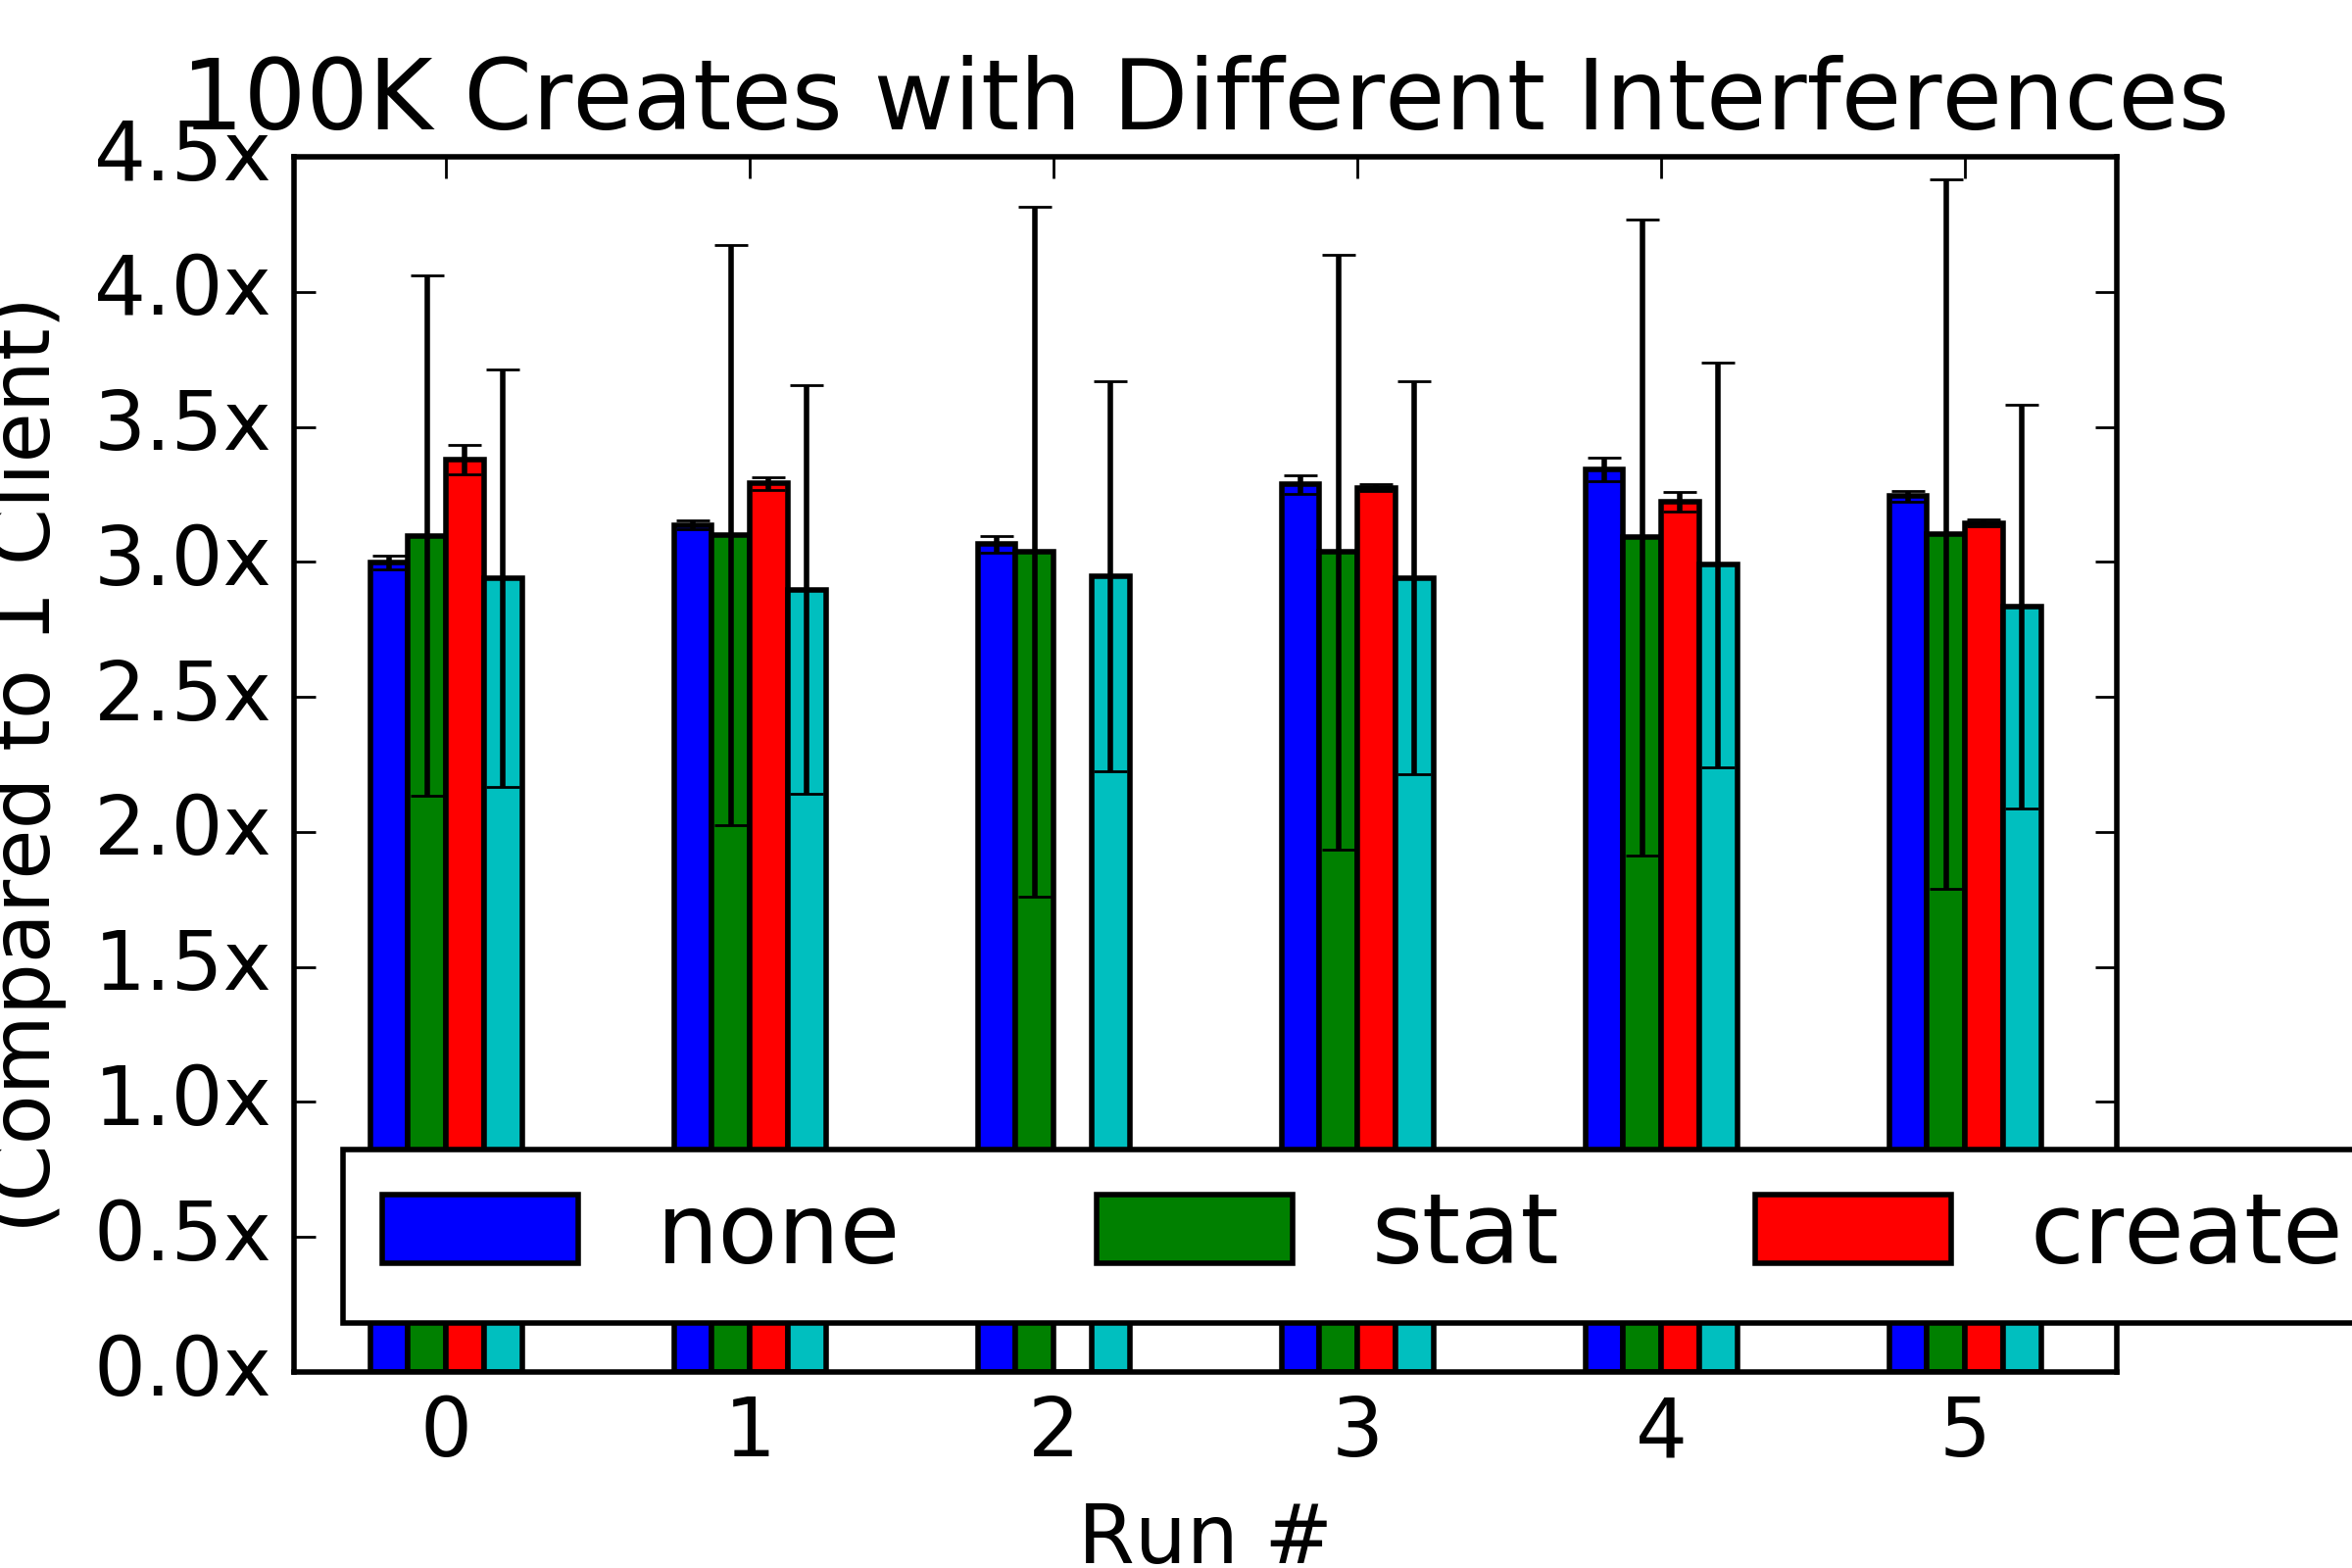
\includegraphics[width=1.0\linewidth]{graphs/slowdown-interfere-types.png}
      \caption{Different interferring requests}
      \label{fig:interfere-c}
  \end{subfigure}
  \caption{When a client create stream is ``isolated" lookups resolve
  locally; but when a second client ``interferes" by creating in the same
  directory, the directory inode capability is revoked forcing all clients to
  centralize lookups at the metadata server.
  \label{fig:interfere}}
\end{figure*}

% inode cache - reduces RPCs (lookups for create, readdirs for stats)
To keep track of the read caching and write buffering capabilities, the clients
and metadata servers agree on the state of each inode using an inode cache.  If
a client has the directory inode cached it can do metadata writes ({\it e.g.},
create) with a single RPC. If the client is not caching the directory inode
then it must do an extra RPC to determine if the file exists.  Unless the
client immediately reads all the inodes in the cache ({\it i.e.} \texttt{ls
-alR}), the inode cache is less useful for create-heavy workloads.

% benefits PROBLEM -- IS THIS THE METADATA PROTOCOL OR JUST THE OVERLOADEDNESS?
The benefits of caching the directory inode when creating files is shown in
Figure~\ref{fig:interfere-a}.  If only one client is creating files in a
directory (``isolated" curve on \(y1\) axis) then that client can lookup the
existence of new files locally before issuing a create request to the metadata
server. If another client starts creating files in the same directory
(``interfere" curve on \(y1\) axis) then the directory inode transitions out of
read caching and the first client must send \texttt{lookup()}s to the metadata
server (``interfere" curve on \(y2\) axis). These extra requests increase the
throughput of the ``interfere" curve because the metadata server can handle the
extra load but the overall performance decreases.  This degradation is shown in
Figure~\ref{fig:interfere-b}, where we scale the number of clients and show
increased runtime and variability. The performance is compared to a single
isolated client and the error bar is the standard deviation of the runtime of
all clients.  For the ``interfere" bars, each client creates files in private
directories and at 30 seconds we launch another process that creates files in
those directories.  For less than 7 clients, the runtime and deviation is worse
when clients interfere. At 7 clients, the metadata server is overloaded so the
directory caching in the ``isolated" bars has no benefit. Zooming in on runs
with 7 clients in Figure~\ref{fig:interfere-c} we see how different
interfering operations affect performance, again when compared to the
performance of a single isolate client.  ``create" has little effect but
``stat" and ``create many" cause noticeable slowdowns because of the extra work
they impose on the metadata server.\\

% TODO: what is the cost of trimming the cache?
% TODO: does CephFS still cache inodes when I turn off caching? Why is still keeping inodes in memory? Gah!

\noindent\textbf{Comparison to decoupled namespaces}: Decoupled namespaces
merge batches of metadata operations into the global namespaces when the job
completes.  In BatchFS the merge is delayed by the application using an API to
switch between asynchronous to synchronous mode. The merge itself is explicitly
managed by the application but future work looks at more automated
methodologies. In DeltaFS snapshots of the metadata subtrees stays on the client
machines; there is no ground truth and consistent namespaces are constructed
and resolved at application read time or when a 3rd party system ({\it e.g.},
middleware, scheduler, etc.) needs a view of the metadata. As a result, all the
overheads of maintaining consistency that we showed above are delayed until the
merge phase.
